\documentclass[preview]{standalone}
\usepackage{tikz}
\usepackage{avant}
\renewcommand*\familydefault{\sfdefault}
\usepackage[T1]{fontenc}
\usetikzlibrary{positioning, backgrounds, shapes, chains, arrows, decorations.pathmorphing, matrix, fit}



\begin{document}

  \begin{center}
    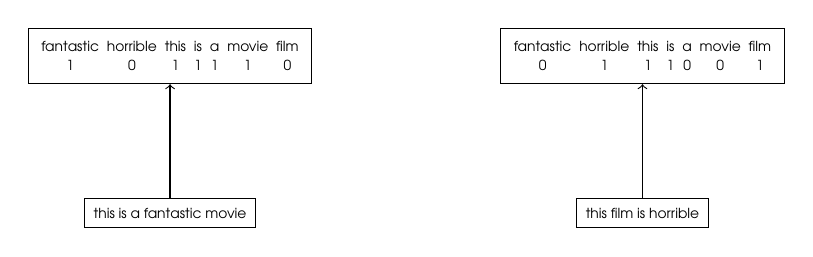
\begin{tikzpicture}
    \node[rectangle, draw] (text1) at (0, 0) {\textsf{\tiny this is a fantastic movie}};
    \node[rectangle, draw] (text2) at (6, 0) {\textsf{\tiny this film is horrible}};

    \begin{scope}[ampersand replacement=\&]
      \matrix (v1) [draw, every node/.style={inner sep=0.5mm}, matrix of nodes, nodes in empty cells, execute at empty cell=\node{\strut}] at (0, 2){
        \textsf{\tiny fantastic} \& \textsf{\tiny horrible }\& \textsf{\tiny this} \& \textsf{\tiny is }\& \textsf{\tiny a} \& \textsf{\tiny movie} \& \textsf{\tiny film}\\ 
        \tiny 1 \& \tiny 0 \& \tiny 1 \& \tiny 1 \& \tiny 1 \& \tiny 1 \& \tiny 0\\
      };
      \matrix (v2) [draw, every node/.style={inner sep=0.5mm}, matrix of nodes, nodes in empty cells, execute at empty cell=\node{\strut}] at (6, 2){
        \textsf{\tiny fantastic} \& \textsf{\tiny horrible} \& \textsf{\tiny this} \& \textsf{\tiny is} \& \textsf{\tiny a} \& \textsf{\tiny movie} \& \textsf{\tiny film}\\ 
        \tiny 0 \& \tiny 1 \& \tiny 1 \& \tiny 1 \& \tiny 0 \& \tiny 0 \& \tiny 1\\
      };
      \path (text1) edge[->] (v1);
      \path (text2) edge[->] (v2);
    \end{scope}
    \end{tikzpicture}
    $\displaystyle \tiny \textsc{Voc} = \{\textsf{\tiny fantastic, horrible, this, is, a, movie, film}\}$
  \end{center}

\end{document}
